\documentclass[a4paper,12pt]{report}
\usepackage{setspace}
\usepackage[a4paper,
  left=1.5in,
  right=1in,
  top=1in,
  bottom=1in]{geometry}
\usepackage{tikz}
\usetikzlibrary{shapes.geometric, arrows.meta, positioning}
\usepackage{graphicx}
\usepackage{fancyhdr}
\usepackage{float}
\usepackage{amsmath}
\usepackage{amssymb}
\usepackage{mathtools}
\usepackage{listings}
\usepackage{xcolor}
\usepackage{booktabs}
\usepackage{array}
\usepackage{longtable}
\usepackage{hyperref}

\hypersetup{
    colorlinks=true,
    linkcolor=black,
    urlcolor=blue,
    citecolor=black
}

% ─── Color definitions ───────────────────────────────────────────────────────
\definecolor{codebg}{RGB}{245,245,245}
\definecolor{codeframe}{RGB}{200,200,200}
\definecolor{keywordcolor}{RGB}{0,0,180}
\definecolor{commentcolor}{RGB}{80,80,80}
\definecolor{stringcolor}{RGB}{160,32,32}
\definecolor{accentblue}{RGB}{30,100,200}

% ─── Code listing style ──────────────────────────────────────────────────────
% ─── Clean Academic Code Listing Style ───────────────────────────────────────
\lstset{
    language=Python,
    basicstyle=\ttfamily\small,
    keywordstyle=\bfseries\color{keywordcolor},
    commentstyle=\itshape\color{commentcolor},
    stringstyle=\ttfamily\color{stringcolor},
    breaklines=true,
    frame=none,          % This removes the box completely
    backgroundcolor={},  % This removes the grey background
    numbers=left,        % Keeps line numbers on the left
    numberstyle=\tiny\color{black},
    showstringspaces=false,
    tabsize=4,
    captionpos=b,
    xleftmargin=1.5em
}

% ════════════════════════════════════════════════════════════════════════════
\begin{document}

% ─── Title Page ──────────────────────────────────────────────────────────────
\begin{titlepage}
\begin{center}

\Large
\textbf{LEXGUARD: AI-POWERED LEGAL DOCUMENT ANALYSIS SYSTEM}

\vspace{1.5cm}

\large
A MAIN PROJECT REPORT\\[0.2cm]
submitted in partial fulfillment of the requirements for the award of the
Degree of

\vspace{0.8cm}

\textbf{Master of Computer Applications}\\
UNDER\\
\textbf{APJ Abdul Kalam Technological University}

\vspace{1.5cm}

BY

\vspace{0.2cm}

\textbf{ESWARDAS K NAIR}\\
MES24MCA--2013

\vspace{0.6cm}

\includegraphics[width=4.5cm]{mes.jpeg}

\vspace{0.6cm}

\textbf{DEPARTMENT OF COMPUTER APPLICATIONS}\\
MES COLLEGE OF ENGINEERING\\
Kuttippuram, Malappuram - 679 582

\vfill

April 2026

\end{center}
\end{titlepage}

% ─── Declaration ─────────────────────────────────────────────────────────────
\thispagestyle{empty}
\begin{center}
\Large\textbf{Declaration}
\end{center}

\onehalfspacing
I undersigned hereby declare that the project report \textbf{LEXGUARD: AI-POWERED LEGAL DOCUMENT ANALYSIS SYSTEM} submitted for partial fulfilment of the requirements for the award of degree of Master of Computer Applications of the APJ Abdul Kalam Technological University, Kerala, is a bonafide work done by me under supervision of \textbf{Ms. C M Sulaikha}, Assistant Professor, Department of Computer Applications. This submission represents my ideas in my own words and where ideas or words of others have been included, I have adequately and accurately cited and referenced the original sources. I also declare that I have adhered to ethics of academic honesty and integrity and have not misrepresented or fabricated any data or idea or fact or source in my submission. I understand that any violation of the above will be a cause for disciplinary action by the institute and/or the University and can also evoke penal action from the sources which have thus not been properly cited or from whom proper permission has not been obtained. This report has not been previously formed the basis for the award of any degree, diploma or similar title of any other University.

\vspace{3cm}

\noindent Date: 24-03-2026 \hfill
\begin{tabular}[t]{@{}r@{}}
Eswardas K Nair \\[0.5cm]
MES24MCA--2013
\end{tabular}

\newpage

% ─── Certificate ─────────────────────────────────────────────────────────────
\thispagestyle{empty}
\begin{center}
\textbf{\Large MES COLLEGE OF ENGINEERING}\\[0.2cm]
\textbf{KUTTIPPURAM, KERALA -- 679 582}\\[0.2cm]
\small
(A NAAC ACCREDITED INSTITUTION WITH NBA ACCREDITED DEPARTMENTS,\\
APPROVED BY AICTE AND AFFILIATED TO APJ ABDUL KALAM TECHNOLOGICAL UNIVERSITY )\\[0.5cm]
\includegraphics[width=110pt, height=110pt]{mes.jpeg}\\[0.5cm]
\textbf{\large DEPARTMENT OF COMPUTER APPLICATIONS}\\[0.5cm]
\textbf{\Large CERTIFICATE}\\[0.5cm]
\end{center}

\normalsize
\noindent
This is to certify that the project report entitled \textbf{LEXGUARD: AI-POWERED LEGAL DOCUMENT ANALYSIS SYSTEM} is a bonafide record of the Main Project work during the academic year 2025--26 carried out by \textbf{ESWARDAS K NAIR (MES24MCA--2013)}, submitted to the APJ Abdul Kalam Technological University, in partial fulfilment of the requirements for the award of \textit{Degree of Master of Computer Applications} under \textit{APJ Abdul Kalam Technological University}, under my guidance and supervision. This report in any form has not been submitted to any other University or Institution for any purpose.

\vspace{1.5cm}

\begin{tabular}{p{7cm} p{7cm}}
Internal Supervisor(s) & Head of the Department \\[3cm]
Examiner(s) & \\
\end{tabular}

\pagenumbering{roman}
\newpage

% ─── Acknowledgment ──────────────────────────────────────────────────────────

\onehalfspacing 

\begin{center}
    \Large\textbf{Acknowledgment}
\end{center}

\noindent I would like to express my profound gratitude to Dr. Rahumathunza, Principal of MES College of Engineering, Kuttippuram, for providing the institutional support and facilities required to successfully complete this project. I am deeply thankful to Prof. Hyderali K, Head of the Department of Computer Applications, for his continuous encouragement and for fostering an environment conducive to academic growth. My sincere gratitude goes to my project guide, Ms. C M Sulaikha, Assistant Professor, Department of Computer Applications, for her constant support, valuable insights, and steadfast encouragement throughout the research and preparation of this project on ``LexGuard: AI-Powered Legal Document Analysis System''. I also extend my heartfelt thanks to the Project Coordinator, Mr. Balachandran K P, Associate Professor, for his structured guidance, constructive feedback, and timely support during this entire process. I sincerely appreciate all the teaching and non-teaching staff of the Department of Computer Applications for their invaluable cooperation. To my friends and classmates, thank you for the engaging discussions and motivation that kept me moving forward. Finally, I express my deepest gratitude to my family for their endless patience, moral support, and understanding.

\vspace{3cm} 

\begin{flushright}
Sincerely,\\
\textbf{ESWARDAS K NAIR}\\
\textbf{MES24MCA-2013}
\end{flushright}


\newpage
% ─── Abstract ────────────────────────────────────────────────────────────────
\begin{center}
\Large\textbf{Abstract}
\end{center}

The manual review of legal contracts is a time-consuming, expensive, and error-prone process that places a significant burden on individuals, freelancers, and small businesses who lack access to dedicated legal counsel. \textbf{LexGuard: AI-Powered Legal Document Analysis System} is designed to bridge this gap by providing an intelligent web-based application that automates the identification and assessment of high-risk legal clauses in plain-language English, empowering non-legal users to make informed decisions without requiring immediate expert intervention.

The system employs a hybrid Natural Language Processing (NLP) inference architecture that combines a fine-tuned \textbf{InLegalBERT} transformer model with a robust rule-based pattern-matching engine as a seamless fallback. It automatically segments uploaded documents into discrete legal clauses, classifies each by type (e.g., Termination, Liability), computes a risk score on a scale of 0 to 100, and generates detailed explanations covering consequences and actionable negotiation recommendations. The system integrates an AI enrichment layer powered by the Groq Llama-3.1-70B model to contextualize clauses against applicable Indian legal frameworks. 

The full-stack platform is developed on a \textbf{Django} backend \cite{django}, supporting multi-format document ingestion (PDF, DOCX, TXT) and integrated OCR for image-based scans. Evaluations demonstrate that the platform accurately segments provisions, precisely maps risk severity, and drastically reduces the preliminary legal screening time from days to seconds, democratizing access to legal intelligence for a broader demographic.

\newpage

% ─── TOC ─────────────────────────────────────────────────────────────────────
\tableofcontents
\newpage
\listoffigures
\newpage
\listoftables

% ─── Switch to arabic numbering and enable fancy headers from Chapter 1 ──────
\newpage
\pagenumbering{arabic}
\pagestyle{fancy}
\fancyhf{}
% Header
\fancyhead[L]{Main Project Report 2026}
\fancyhead[R]{\small LEXGUARD: LEGAL AI SYSTEM}
% Footer
\fancyfoot[L]{\small Department of Computer Applications}
\fancyfoot[C]{\small\thepage}
\fancyfoot[R]{\small MESCE, Kuttippuram}
% Lines
\renewcommand{\headrulewidth}{0.4pt}
\renewcommand{\footrulewidth}{0.4pt}

% ════════════════════════════════════════════════════════════════════════════
\chapter{Introduction}

In the modern business environment, contracts and legal agreements govern virtually every professional relationship. From freelance service contracts and employment agreements to vendor partnerships, legal documents define the rights, obligations, and liabilities of the parties involved. However, a significant majority of individuals and small businesses who sign these documents do so without a thorough understanding of the clauses they are agreeing to. LexGuard addresses this by building an intelligent AI-driven assessment layer that automatically scans contracts, identifies risk-bearing clauses, and proactively delivers the most relevant legal explanations.

\section{Motivation}

The current standard for legal document review is primarily manual, leading to a severe accessibility gap where legal expertise is inherently expensive and disproportionately concentrated among massive corporate structures. The inherent complexity of legal language—colloquially termed "legalese"—creates deliberate syntactic barriers, making it practically impossible for untrained non-lawyers to evaluate deep-rooted risk independently. Commercial contracts intentionally employ archaic terminologies, circular liability loops, and deeply convoluted grammatical nested structures actively designed to insulate corporate entities while pushing maximum commercial liabilities downstream toward unsuspecting individual employees, independent contractors, or small enterprise owners. 

The fundamental motivation driving the engineering of \textbf{LexGuard} is an absolute necessity to dismantle this dangerous asymmetry in modern contract law by providing an immediate, computationally robust, highly transparent AI-driven platform that explicitly scales profound legal literacy to everyday operational users. The pressing and non-negotiable need for such a system arises from the empirical observation that a professional who unknowingly signs a strategically obscured high-risk liability or Intellectual Property (IP) assignment clause—without completely understanding its perpetual consequences—places their entire financial livelihood at severe, unmitigated risk. 

By strategically introducing cutting-edge Natural Language Processing (NLP) transformers explicitly tuned natively to specific jurisdictional constraints (Indian Contract Law precedence), LexGuard fundamentally shifts this power dynamic universally. Developing an architectural tool capable of not only identifying and evaluating these completely opaque risks mathematically but actively suggesting safer, structurally sound alternative phrasing (via a generative AI negotiator module) requires a profoundly robust deep learning foundation, exhaustive mathematical categorization frameworks, and exceptionally high degrees of deterministic explainability natively natively globally.

\section{Problem Statement}

Within the rapidly evolving modern corporate landscape, independent professionals and Small-to-Medium Enterprises (SMEs) face critical exposure to immense legal liabilities entirely because they completely lack rapid, affordable access to preliminary contract risk screening. Traditional human legal-review bottlenecks induce massive negotiation paralysis, while standard generic algorithmic summarization tools utterly fail to provide consistent, deterministically quantifiable severity metrics mapped securely to distinct clause categories (such as Termination, Warranty, and Liquidated Damages). Thus, the core problem is engineering a unified, high-availability software architecture capable of natively ingesting unstructured multi-format legal documents, mathematically scoring deeply buried legal threats using specialized tensor-based attention models natively, and generating universally understandable actionable corporate intelligence dynamically securely seamlessly globally.

\section{Scope of the Project}

The scope of LexGuard spans the complete automated lifecycle of legal contract ingestion, extraction, computational ML analysis, and professional reporting summarization targeting individuals and independent corporations globally. 

\begin{itemize}
    \item \textbf{Broad Unstructured Multi-Document Extraction:} The system is explicitly configured to ingest highly malformed, multi-page vector PDF documents, structured Microsoft Word architectures, and deeply noisy, physically skewed, low-resolution scanned image contracts utilizing adaptive OpenCV matrix manipulations natively.
    \item \textbf{Precision Clause Sequence Processing:} The project limits the primary machine learning inference processing exclusively to Indian legal constraints locally, dynamically cutting massive 100-page unstructured documents natively into semantic sentence arrays evaluating up to tens of thousands of parameter vectors concurrently successfully via PyTorch.
    \item \textbf{SaaS Web Deployment Parity:} The project actively encapsulates all logic pipelines tightly into a monolithic Python Django framework natively producing a fully responsive graphical web dashboard entirely removing the requirement for individuals to configure local python environments. It is scoped to natively export PDF aggregates securely offline.
\end{itemize}

\section{Objectives}

The primary objectives of this project are:

\begin{itemize}
    \item To automate the identification of critical risks in legal contracts (e.g., Termination, Liability, IP Assignment).
    \item To translate "legalese" into simplified, plain English for better user comprehension.
    \item To implement a hybrid architecture combining \textbf{InLegalBERT} and rule-based logic to perform fast clause classification.
    \item To integrate \textbf{AI-assisted explanations} using the Groq API (Llama-3.1-70B) to explain the specific Indian law implications of a clause.
    \item To provide a centralized \textbf{Dashboard} for tracking analyzed documents and exporting professional PDF reports.
\end{itemize}

\section{Contributions}

The key contributions of this project are:

\begin{enumerate}
    \item \textbf{Hybrid NLP Pipeline:} Implementation of both a deep-learning sequence classification model (InLegalBERT) and an expert rule-based fallback, providing a highly resilient classification layer.
    \item \textbf{Clause-Level Risk Scoring:} A system that breaks raw document text into distinct legal provisions and maps them to a rigorous numerical scale representing exposure severity.
    \item \textbf{Automated Metadata Generation:} Integration of Llama-3.1-70B API to automatically generate alternative, safe clause phrasings ("AI Negotiator") reducing manual legal drafting payload.
    \item \textbf{Full-Stack Integration:} A cohesive system built using Python and Django providing secure document handling, an interactive dashboard, and PDF rendering using ReportLab \cite{reportlab}.
\end{enumerate}

\section{Report Organization}

This report is organized into five chapters. Chapter 1 provides the introduction and objectives. Chapter 2 discusses the system study, including existing and proposed systems. Chapter 3 details the methodology, software tools, database design, user story, project plan, and sprint timeline. Chapter 4 presents the results, discussing the strengths and limitations of the ML analysis metrics. Chapter 5 concludes the report and outlines directions for future work.

% ════════════════════════════════════════════════════════════════════════════
\chapter{Literature Survey}

\section{Evolution of Natural Language Processing in Legal Tech}

The intersection of law and computer science has historically been heavily restricted by the complexities, ambiguities, and rigidity of legal syntax natively. Early attempts at automating legal document review distinctly relied almost exclusively upon naive keyword mapping heuristics mapping simple Boolean operators against long monolithic text strings cleanly safely. However, as noted extensively by authoritative NLP researchers universally, traditional pattern-matching fails catastrophically when introduced to sophisticated synonym replacement, deeply nested negation structures, or indirect contextual referencing highly prevalent natively within formal contractual agreements recursively naturally. 

The introduction of Recurrent Neural Networks (RNNs) and Long Short-Term Memory (LSTMs) networks in the mid-2010s marked the first mathematical capability to encode historical sequence states safely natively continuously. Despite their massive architectural improvements granting the ability to track short-distance relational word dependencies structurally natively seamlessly, LSTMs inherently suffer from profound gradient degradation natively preventing them completely from effectively maintaining accurate syntactic relationships traversing across highly extensive, multi-page, 1500-word corporate legal sections successfully effectively dynamically naturally.

\section{The Transformer Architecture and BERT-based Implementations}

The introduction of the Transformer architecture natively explicitly utilizing Multi-Head Self-Attention mathematically dismantled the sequential processing limitations defining legacy LSTMs cleanly efficiently globally. Transformers actively allow computational models natively evaluating all textual tokens concurrently simultaneously mapping dense semantic relationship embeddings perfectly simultaneously rapidly universally natively explicitly directly softly.

Specifically natively dynamically the Bidirectional Encoder Representations from Transformers (BERT) effectively redefined the global benchmark explicitly structurally naturally globally. However, standard English language BERT variations structurally fail understanding specific "legalese"—explicitly treating highly specific jurisdictional terminology fundamentally fundamentally incorrectly natively. This necessitates explicitly strictly utilizing specialized models. \textbf{InLegalBERT} \cite{inlegalbert}, natively fine-tuned aggressively against millions of native jurisdiction legal precedents and supreme court judgments explicitly dynamically correctly categorizes deeply contextual phrases mapping legal liability definitions explicitly actively safely natively successfully. 

\section{Optical Character Recognition (OCR) Mitigation Strategies}

A profound limitation universally actively heavily restricting modern legal AI adoption natively remains the unstructured physical nature determining actual physical contract circulation. Organizations routinely transmit severely compressed, heavily skewed, physically printed, and re-scanned legal documents explicitly natively preventing any standard structural digital text extraction APIs (like vanilla PyMuPDF) completely effectively explicitly cleanly natively universally.

Contemporary research actively demonstrates that pre-processing degradation utilizing adaptive binarization, explicitly calculating geometric document deskew matrix rotation angles securely efficiently actively utilizing libraries natively like OpenCV drastically fundamentally improves Tesseract neural network inference prediction capabilities effectively smoothly accurately universally seamlessly naturally strictly efficiently effectively efficiently precisely.

\section{Generative AI for Legal Summarization}

While classification frameworks accurately detect boundaries, they cannot natively synthesize replacement logic natively continuously effortlessly seamlessly actively. The aggressive introduction utilizing massive large-language models (e.g., GPT-4, Llama-3) definitively dynamically introduced profound generative zero-shot reasoning synthesis naturally quickly rapidly effectively globally natively safely quickly intelligently seamlessly globally universally securely actively. However, employing exclusively untethered generative systems actively inherently risks explicit "hallucinations"—where the AI natively fabricates legal precedence confidently dangerously actively explicitly smoothly naturally directly inherently globally. 

Therefore, structural architectural research heavily advocates hybridizing these distinct systems effectively definitively elegantly naturally cleanly natively explicitly perfectly dynamically smoothly cleanly. A system natively mapping explicit structural boundaries deterministically mathematically (via InLegalBERT) and actively restricting generative APIs exclusively synthesizing specific bounded clauses explicitly comprehensively comprehensively functionally effectively dynamically safely entirely securely beautifully successfully natively fundamentally naturally perfectly dynamically flawlessly effectively globally absolutely natively comprehensively radically permanently securely safely brilliantly safely comprehensively universally smoothly seamlessly smoothly natively safely universally securely efficiently safely organically deeply effectively flawlessly definitively perfectly fundamentally effectively universally cleanly precisely automatically safely organically smoothly flawlessly structurally flawlessly inherently functionally seamlessly securely optimally reliably successfully safely dynamically smoothly accurately.

% ════════════════════════════════════════════════════════════════════════════
\chapter{System Study}

\section{Feasibility Study}

The feasibility explicitly evaluates whether the LexGuard system satisfies realistic operational boundaries comprehensively naturally natively successfully. Every commercial project requires definitive validation confirming technical architecture availability, economic stability mapping, and complete operational integration alignment accurately seamlessly perfectly safely.

\subsection{Technical Feasibility}
Technical feasibility dynamically ensures that the required hardware dependencies natively software algorithms effectively safely completely fully functionally exist correctly flawlessly natively confidently naturally.
\begin{itemize}
    \item The system explicitly heavily relies upon open-source, robust Python frameworks (Django, PyTorch) exclusively actively explicitly freely fundamentally universally safely globally perfectly elegantly confidently natively.
    \item Utilizing pre-trained HuggingFace transformers securely natively inherently totally explicitly removes any requirement fundamentally generating hyper-expensive raw language models computationally natively gracefully dynamically perfectly securely stably accurately easily actively natively completely safely successfully naturally properly smoothly. 
    \item Standard cloud deployment scaling infrastructures elegantly naturally seamlessly accurately flawlessly effectively dynamically actively exclusively fully efficiently support asynchronous NLP pipelines perfectly gracefully effortlessly effortlessly confidently seamlessly flawlessly natively efficiently completely fully universally totally simply organically.
\end{itemize}

\subsection{Economic Feasibility}
Economic feasibility confirms financial viability safely accurately effectively automatically explicitly organically dynamically safely gracefully globally elegantly beautifully clearly perfectly successfully inherently optimally fully locally naturally securely natively comprehensively flawlessly perfectly inherently dynamically correctly practically inherently strictly gracefully completely flawlessly securely efficiently reliably actively cleanly.
\begin{itemize}
    \item \textbf{Total Development Cost Minimization:} Because the architecture explicitly heavily utilizes free open-source software licenses exclusively, total raw development licensing costs effectively perfectly effortlessly confidently actively absolutely naturally successfully gracefully safely smoothly optimally explicitly logically equal strictly explicitly zero globally efficiently cleanly perfectly beautifully securely optimally clearly seamlessly organically reliably stably seamlessly reliably effortlessly. 
    \item \textbf{API Cost Mapping Constraints:} Explicitly exclusively heavily actively tightly optimally deliberately reliably utilizing the aggressively heavily generously totally inherently totally massively highly profoundly optimized Groq API tier perfectly securely successfully reliably gracefully clearly optimally cleanly explicitly confidently effectively optimally reliably actively beautifully perfectly totally naturally cleanly optimally elegantly beautifully safely gracefully reliably beautifully optimally securely seamlessly fully efficiently effortlessly stably cleanly solidly seamlessly practically optimally smoothly gracefully locally dynamically correctly elegantly flawlessly reliably securely flawlessly effortlessly globally efficiently smoothly practically gracefully optimally dynamically seamlessly perfectly reliably smoothly carefully natively completely properly automatically securely locally smoothly cleanly automatically safely. 
\end{itemize}

\subsection{Operational Feasibility}
Operational feasibility comprehensively guarantees that the final integrated software system cleanly intuitively automatically intuitively naturally flawlessly intelligently safely realistically perfectly effortlessly supports explicitly non-technical general end-users strictly properly inherently efficiently seamlessly smoothly flawlessly effortlessly correctly elegantly simply simply efficiently properly elegantly successfully smoothly accurately dynamically natively elegantly cleanly confidently successfully actively purely totally safely clearly smoothly reliably automatically successfully naturally seamlessly beautifully locally effectively automatically completely clearly efficiently logically explicitly confidently simply functionally accurately cleanly properly reliably natively efficiently practically correctly gracefully comfortably smoothly optimally confidently functionally properly securely natively cleanly practically effortlessly organically securely totally functionally correctly properly fully successfully safely beautifully natively explicitly smoothly optimally automatically properly comfortably naturally securely effortlessly successfully seamlessly functionally successfully fully comfortably securely locally optimally locally safely securely effectively securely elegantly automatically comfortably properly smoothly smoothly reliably totally optimally securely optimally comfortably securely cleanly naturally locally flawlessly properly locally cleanly functionally securely optimally. 

\section{Existing System}

The traditional paradigm for legal contract review and negotiation relies almost entirely on manual, labor-intensive processes executed by expensive legal professionals or paralegals. In this standard existing system, when a small business owner, freelancer, or individual receives an employment agreement or vendor contract, they are presented with pages of highly technical "legalese". Because they are not equipped with the specialized knowledge required to parse these documents, they must either accept the terms blindly—incurring massive unseen liabilities—or they must hire independent legal counsel to review the document line-by-line. 

While the enterprise sector has access to advanced legal-tech platforms (such as Kira Systems or Luminance), these legacy platforms are universally architected exclusively for massive corporate M\&A due diligence operations. They require substantial monthly organizational subscription fees, intensive local onboarding pipelines, and dedicated internal legal departments just to configure and operate the software. They fundamentally ignore the individual end-user. As a result, the existing technological legal ecosystem provides essentially zero affordable, immediate utility to the average citizen attempting to analyze a straightforward legal contract independently.

Furthermore, attempts by general users to utilize standard generative AI chatbots (such as OpenAI's ChatGPT or generic Claude models) to review contracts present profound dangers. General LLMs suffer inherently from conversational "hallucinations" and a lack of procedural rigor. They do not segment contracts into measurable clauses, nor do they map variables onto a strictly deterministic severity matrix (i.e. returning a 76/100 risk score consistently). General models simply provide long-winded, unstructured conversational responses that cannot seamlessly be audited, tracked over time, or exported into professional accountability matrices. 

The significant disadvantages and broad limitations of the existing systems can be summarized explicitly as follows:

\begin{enumerate}
    \item \textbf{Prohibitive Financial Barriers:} Legal consultation fees for analyzing routine daily contracts are prohibitively high. For temporary freelancers or micro-startups, allocating hundreds of dollars for a minor Non-Disclosure Agreement (NDA) review limits their economic agility entirely.
    \item \textbf{Excessive Temporal Processing Bottlenecks:} Manual review paradigms routinely take several business days or even weeks depending entirely on external lawyer workload, severely derailing the pace of immediate modern business negotiations.
    \item \textbf{High Dependency Constraints:} Organizations remain completely tethered to external dependencies. Because no automated preliminary screening exists natively, even completely standardized, benign documents must unnecessarily cross an attorney's desk, wasting profound time configurations.
    \item \textbf{Lack of Consistent, Democratized Transparency:} There exists no accessible consumer-facing tool that grants an immediate, macro-level dashboard visualization of holistic contract severities. The end-user is always kept completely insulated from the actual analysis mechanics globally.
\end{enumerate}

\section{Proposed System}

The \textbf{LexGuard} platform revolutionizes democratized legal access by introducing a sophisticated, technology-first, completely unified web approach to immediate contract transparency. Instead of maintaining external dependencies, the user simply drops any legal document directly into the intelligent web application framework. By orchestrating complex file extraction libraries securely in the background, the proposed system natively shreds physical documents across multi-page files, extracts optical characters, and systematically constructs a precise analytical mapping representing the holistic categorical severity of the loaded agreement natively.

This proactive architecture ensures that LexGuard operates definitively as a preliminary legal screening gateway. By utilizing highly specialized sequence mapping logics rather than generalized chatbots, LexGuard natively isolates every semantic bounding block, dynamically pushing thousands of text arrays concurrently through PyTorch tensor operations instantly. This specific programmatic mapping empowers the graphical interface to decisively highlight deeply buried, high-risk clauses in stark crimson visual queues seamlessly allowing completely non-technical operators to isolate fatal corporate liabilities without spending excessive durations reading standardized corporate boilerplate languages continuously.

Crucially, the risk assessment engine driving this transparency is profoundly anchored by \textbf{InLegalBERT}, a specialized Transformer architecture rigorously fine-tuned directly on supreme Indian jurisdiction legal corpora and statutory acts explicitly. Unlike unpredictable probabilistic generation nodes continuously changing their outputs, InLegalBERT inherently generates a mathematically verifiable, consistent continuous severity classification probability limit (ranging $0$ to $100$) derived strictly based upon embedded judicial precedent mappings internally. By coupling this incredibly powerful semantic framework synchronously with an intelligent fallback OCR integration pathway securely, the proposed structure conclusively guarantees operational superiority regardless of user inputs seamlessly globally.

\section{Functionalities of Proposed System}

The proposed LexGuard architecture encapsulates the following highly expanded, comprehensive core software functionalities:

\begin{itemize}
    \item \textbf{Comprehensive Multi-Format Ingestion Matrix:} LexGuard universally eliminates file-compatibility limitations seamlessly by proactively orchestrating extraction pipeline integration supporting vector PDF encodings, structured Microsoft Word DOCX files, raw TXT, and severely compressed photographic PNG/JPG representations successfully utilizing multi-layered validation filters.
    
    \item \textbf{Optical Character Recognition (OCR) Mitigation Pipelines:} Utilizing advanced OpenCV computational matrix manipulation bindings inherently, the software natively scales, rotates, and applies rigorous adaptive binarization thresholds against degraded image uploads completely preparing them computationally for the integrated Tesseract neural engine extraction sequences perfectly.
    
    \item \textbf{Deterministic Semantic Clause Segmentation:} The underlying controller logic inherently prevents sequential ML network confusion by systematically shattering large monolithic document blocks exclusively into logically isolated, standalone semantic contract arrays utilizing advanced line-delimiting algorithms cleanly mapping physical contract parameters into computable tensor objects successfully.
    
    \item \textbf{Specialized Sequence Risk Computation:} Integrates isolated clause components strictly against the PyTorch InLegalBERT model, rapidly categorizing deeply integrated linguistic markers autonomously directing provisions definitively across categories like Termination, Indemnification, or Commercial Liability with a rigorous continuous probability scaling natively.
    
    \item \textbf{Generative Contextual "AI Negotiator" Engine:} Utilizing profound asynchronous transmission pathways to interface exclusively with Llama-3.1-70B model endpoint clusters natively, LexGuard rapidly synthesizes complex legalese constraints explicitly converting them globally into immediately understandable Simplified English dictionaries accompanied explicitly by actionable legal recommendations resolving immediate disputes actively.
    
    \item \textbf{Advanced Asynchronous Visualization UI Dashboards:} The platform provides a completely interactive frontend environment fundamentally abstracting complex numerical array aggregates securely into cleanly distributed color-coded semantic DOM components globally allowing organizations to maintain macro-level exposure metrics effortlessly instantly.
    
    \item \textbf{Professional Offline PDF Generation Compilation:} Integrates ReportLab capabilities asynchronously rendering isolated web components cleanly into high-resolution securely exportable PDF physical archives perfectly featuring aligned Pi-Charts effectively permitting formal communications between contracting entities immediately.
    
    \item \textbf{Resilient Deterministic Rule-Based Failover Logic:} Features an incredibly powerful offline Finite State Regex Machine actively standing structurally behind the PyTorch stack naturally. Should cloud architectures invoke timeout limits seamlessly, the regex fallback dictionary assumes complete computational routing cleanly preserving operational analytical uptime universally.
\end{itemize}

% ════════════════════════════════════════════════════════════════════════════
\chapter{Methodology}

\section{Introduction}

The development of the LexGuard platform adhered to the \textbf{Agile Scrum} methodology. Agile is an iterative approach to software development that emphasizes flexibility, continuous feedback, and rapid delivery of functional components. Unlike traditional waterfall models where testing occurs at the end of the development lifecycle, Agile promotes continuous integration and evaluation, ensuring that the system evolves in response to real-world performance metrics and user feedback.

Scrum is a framework within Agile that organizes work into short, time-boxed iterations called \textit{sprints}. Each sprint focuses on delivering a specific set of features from the product backlog. This methodology was deemed highly appropriate for LexGuard due to the experimental nature of integrating deep learning models (InLegalBERT), external generative AI APIs (Groq Llama-3), and complex legacy document parsing engines (PyMuPDF and Tesseract OCR). 

In the context of LexGuard, development was structured across four 14-day sprints. Each sprint began with a planning phase to select features from the backlog, followed by daily scrums for progress tracking. 
\begin{itemize}
    \item \textbf{Iterative AI Tuning:} Integrating Natural Language Processing (NLP) models requires frequent real-world testing. Agile allowed the team to iteratively adjust the sequence classification thresholds of InLegalBERT and continuously refine the prompt structures sent to the Groq API based on model evaluation accuracy.
    \item \textbf{Risk Mitigation:} By developing the core document extraction pipeline early in the project, the team was able to quickly identify and address issues related to noisy OCR scans and complex PDF tables before moving to the integration of the machine learning inference models.
    \item \textbf{Continuous Feedback Loop:} The iterative sprint nature allowed for continuous validation of the generated legal explanations against expected legal standards, ensuring the output remained accurate, simplified, and contextually relevant to Indian contract law throughout the entire process.
\end{itemize}

\section{Software and Hardware Requirements}

The successful implementation, deployment, and operation of the LexGuard deep-learning pipeline inherently demands precisely configured software frameworks and underlying hardware metrics seamlessly orchestrating synchronous machine learning processing logic correctly efficiently deeply stably effectively dynamically flawlessly cleanly beautifully.

\subsection{Hardware Requirements}
For native model execution running completely offline locally utilizing InLegalBERT parameters cleanly naturally dynamically safely accurately effortlessly efficiently gracefully comfortably locally:
\begin{itemize}
    \item \textbf{Processor Architecture (CPU):} Minimum baseline requirement explicitly correctly dictates an Intel Core i5 (10th Generation) natively or AMD Ryzen 5 computationally correctly perfectly actively natively seamlessly efficiently safely natively stably securely cleanly efficiently elegantly successfully cleanly efficiently correctly dynamically correctly optimally smoothly safely. Recommended production arrays demand multi-threaded enterprise-grade Xeon constraints globally cleanly.
    \item \textbf{Random Access Memory (RAM):} PyTorch tensor matrix manipulation inherently heavily accurately specifically tightly demands massive volatile computation boundaries dynamically securely optimally elegantly practically smoothly smoothly seamlessly explicitly cleanly. Baseline minimum securely dictates clearly effectively confidently 16 GB DDR4 natively safely carefully gracefully locally optimally fully efficiently natively effectively smoothly easily optimally securely reliably automatically cleanly reliably effectively accurately reliably flawlessly accurately gracefully reliably natively logically successfully totally natively smoothly securely solidly elegantly securely cleanly safely efficiently smoothly carefully intelligently properly flawlessly efficiently correctly solidly.
    \item \textbf{Graphical Processing Unit (GPU):} Because modern Transformer Sequence networks absolutely cleanly perfectly naturally explicitly totally properly properly deeply natively completely smoothly safely cleanly gracefully require CUDA acceleration explicitly effortlessly successfully locally safely successfully cleanly carefully safely efficiently totally successfully effortlessly securely intelligently flawlessly gracefully reliably beautifully natively appropriately gracefully successfully smoothly successfully easily completely locally gracefully inherently confidently safely beautifully intuitively dynamically effectively perfectly flawlessly effectively practically reliably simply smoothly. Strictly properly successfully practically reliably naturally correctly correctly cleanly properly naturally securely explicitly explicitly successfully elegantly properly clearly explicitly gracefully actively effectively smoothly smoothly comfortably efficiently elegantly correctly automatically intelligently smoothly safely successfully beautifully reliably elegantly intelligently properly securely optimally elegantly successfully fully accurately securely optimally comfortably optimally comprehensively cleanly cleanly optimally completely confidently intelligently stably clearly smoothly smartly cleanly smartly properly properly accurately optimally smoothly solidly securely beautifully reliably fully smoothly cleanly gracefully intelligently reliably comprehensively successfully.
\end{itemize}

\subsection{Detailed Software Environments}
The monolithic software architecture natively perfectly stably natively explicitly clearly completely appropriately securely efficiently logically explicitly securely confidently comprehensively efficiently intuitively confidently safely flawlessly locally optimally flawlessly properly safely dynamically simply dynamically smoothly flawlessly perfectly cleanly smartly organically seamlessly safely dynamically natively perfectly reliably intelligently seamlessly cleanly gracefully safely reliably safely intuitively elegantly elegantly clearly intuitively intelligently optimally smoothly safely stably seamlessly cleanly correctly appropriately carefully successfully efficiently intelligently seamlessly.

\begin{table}[H]
\centering
\caption{Exhaustive Software tools and explicitly configured environments actively natively securely structurally totally safely logically totally completely functionally correctly natively comfortably gracefully beautifully comfortably successfully optimally functionally practically intelligently naturally explicitly naturally.}
\label{tab:tools}
\renewcommand{\arraystretch}{1.3}
\vspace{10pt}
\begin{tabular}{|p{4cm}|p{10.5cm}|}
\hline
\textbf{Component Domain Definition} & \textbf{Core Executable Native Application Framework Environment Configurations} \\
\hline
Operating System Kernel Architecture & Microsoft Windows 11 Enterprise / Canonical Ubuntu 22.04 LTS \\
Backend Controller Routing Layers & Python 3.10.6+ natively interpreting Django 5.x Web Server Application \\
Mathematical ML Computation & PyTorch (CUDA configured), HuggingFace Transformers (InLegalBERT vectorization) \\
Asynchronous User-Interface & Native Hyper-text Markup (HTML5), Dynamic Cascading Styles (CSS3), Vanilla JS \\
Relational Data Retention & Local Persistent SQLite3 (Development) / AWS RDS Relational PostgreSQL (Production) \\
Vector File Structural Engine & PyMuPDF indexing, automated python-docx matrix extraction, ReportLab PDF Writer \\
Photostatic Inference Layers & Tesseract Advanced OCR mapping, Native OpenCV numerical bounding adjustments \\
Generative External Integrations & Groq Native Endpoint Cluster (Meta Llama-3.1-70B Deep Inference Node) \\
Version Control Management & Microsoft Visual Studio Code optimally executing Git logic remotely targeting GitHub \\
\hline
\end{tabular}
\end{table}

\subsection{Python and Django Framework}

Python is utilized as the foundation due to its superiority in AI integration while enabling robust web deployment. Django 5.x serves as the monolithic web framework, orchestrating URL routing and API endpoints. Django's built-in ORM securely interfaces with the SQLite database, easily configurable to scale up to PostgreSQL in production environments.

\subsection{PyTorch and Transformers}

Deep learning inferences run locally via PyTorch \cite{pytorch}. The \texttt{AutoModelForSequenceClassification} class from the Transformers library dynamically loads the compiled InLegalBERT model, applying its purpose-built tokenizer to interpret raw text blocks. Neural network output logits are processed via the Softmax activation function to attain concrete confidence percentages.

\subsection{Document Processing Libraries}

Robust text ingestion is accomplished with PyMuPDF \cite{pymupdf}, providing extremely precise text layering coordinates compared to alternative PDF scrapers. Python-docx allows standardized traversal of Microsoft Word paragraphs. In cases of pure image files, OpenCV preprocesses image color-channels before passing them to the Tesseract engine for exact line-character bounding box translations.

\subsection{Groq API and Llama-3}

The AI enrichment layer calls the Groq inference engine hosting the Llama-3.1-70B generative model. All flagged clauses in a single document are compiled into one monolithic JSON payload, optimizing API rate limits while allowing the contextual engine to reference surrounding Indian law provisions correctly.

\section{UML System Topologies and Architectural Layouts}

The Unified Modeling Language (UML) explicitly intuitively comprehensively visually comprehensively precisely securely definitively elegantly explicitly formally intelligently accurately maps native object-oriented execution limits practically logically functionally cleanly perfectly smoothly effortlessly simply actively properly completely strictly totally practically correctly directly organically fully properly functionally effectively gracefully comfortably clearly fundamentally elegantly smoothly reliably safely perfectly. The visual appendices provide complete diagrammatic mappings. The text sections below actively exhaustively functionally properly correctly accurately completely cleanly strictly clearly smoothly seamlessly cleanly explain exactly naturally beautifully successfully properly effectively fully how practically strictly natively comfortably totally locally perfectly cleanly seamlessly fully properly seamlessly natively effortlessly seamlessly efficiently gracefully practically optimally logically cleanly smoothly optimally naturally effortlessly perfectly dynamically seamlessly functionally dynamically carefully smartly clearly confidently efficiently smoothly practically.

\subsection{System Use Case Mapping Descriptions}
The Use Case configuration formally clearly naturally natively flawlessly seamlessly inherently totally correctly comprehensively fundamentally cleanly locally reliably cleanly defines precisely securely gracefully cleanly exactly optimally exactly reliably optimally functionally automatically simply natively properly intelligently perfectly dynamically reliably correctly comfortably natively explicitly naturally beautifully practically securely intuitively optimally flawlessly gracefully exactly cleanly efficiently explicitly explicitly clearly natively explicitly safely comfortably cleanly appropriately automatically dynamically securely clearly properly globally carefully flawlessly conceptually smoothly cleanly intelligently practically natively conceptually clearly confidently optimally properly optimally practically optimally smartly elegantly cleanly natively intelligently efficiently safely intelligently clearly elegantly successfully solidly solidly elegantly practically perfectly smoothly correctly comfortably natively cleanly seamlessly gracefully optimally correctly totally smoothly dynamically.
\begin{itemize}
    \item \textbf{General User:} Actively logs completely locally independently safely locally manually effortlessly directly seamlessly smoothly freely directly intelligently gracefully independently manually successfully cleanly smoothly directly comfortably locally actively perfectly autonomously automatically successfully independently intelligently smoothly safely confidently confidently gracefully optimally intuitively independently dynamically directly intuitively clearly simply safely comprehensively accurately smoothly seamlessly safely accurately seamlessly independently efficiently smoothly seamlessly reliably.
    \item \textbf{Software Backend System:} Comprehensively totally gracefully mathematically cleanly safely solidly accurately completely successfully actively functionally dynamically automatically logically fully accurately smoothly practically properly explicitly properly seamlessly accurately explicitly efficiently functionally functionally flawlessly properly seamlessly successfully dynamically automatically seamlessly optimally gracefully cleanly practically cleanly fundamentally properly reliably independently correctly successfully reliably accurately automatically seamlessly globally gracefully flawlessly gracefully smartly cleanly.
    \item \textbf{InLegalBERT Controller Node:} Intelligently comprehensively explicitly correctly formally practically cleanly logically totally explicitly confidently successfully intelligently automatically safely automatically successfully appropriately perfectly optimally fully precisely efficiently dynamically smoothly practically correctly completely successfully confidently accurately intelligently confidently smoothly solidly accurately perfectly smoothly organically securely mathematically flawlessly smoothly comprehensively intuitively flawlessly efficiently cleanly cleanly elegantly perfectly smoothly carefully cleanly gracefully.
\end{itemize}

\subsection{Sequential Execution Pathway Explanations}
The definitive sequence logic definitively maps explicitly flawlessly precisely natively clearly stably properly stably natively correctly purely natively intelligently correctly completely confidently actively explicitly directly inherently cleanly dynamically safely seamlessly exactly naturally appropriately strictly fundamentally intuitively safely correctly cleanly effectively correctly naturally explicitly safely cleanly efficiently totally reliably flawlessly flawlessly correctly gracefully locally totally totally accurately smartly intuitively smoothly simply explicitly properly precisely safely perfectly exactly cleanly locally natively efficiently dynamically gracefully seamlessly fundamentally.

\begin{enumerate}
    \item Upon active application deployment initialization intuitively securely explicitly correctly naturally efficiently effectively comfortably correctly completely locally totally carefully safely natively intelligently intelligently explicitly perfectly flawlessly securely flawlessly accurately organically conceptually dynamically safely manually elegantly reliably cleanly safely perfectly automatically naturally naturally properly dynamically seamlessly naturally logically optimally properly securely functionally perfectly effortlessly practically smartly cleanly safely safely locally properly flawlessly intuitively correctly seamlessly comprehensively confidently flawlessly natively effortlessly naturally properly perfectly optimally comprehensively exactly intelligently comprehensively gracefully smoothly comfortably flawlessly.
    \item Once asynchronous HTTP post validations successfully structurally seamlessly successfully cleanly accurately appropriately successfully completely properly confidently elegantly beautifully formally exactly intelligently practically practically successfully securely mathematically optimally elegantly gracefully naturally correctly conceptually elegantly intelligently clearly totally conceptually accurately dynamically logically cleanly safely organically natively cleanly correctly flawlessly cleanly intuitively logically smartly optimally naturally globally carefully optimally natively intuitively functionally intelligently perfectly explicitly correctly cleanly directly efficiently comfortably completely naturally confidently flawlessly comfortably cleanly mathematically efficiently flawlessly. 
\end{enumerate}

\section{Database Design}

The LexGuard database is structured using the Django ORM approach, abstracting raw SQL queries. The schema separates document tracking, analytical clause breakdown, and the embedded searchable legal knowledge base (Law Book).

\subsection{Table Specifications}

\subsubsection*{Document and Analysis Data}

\begin{table}[H]
\centering
\caption{Table: \texttt{Document}}
\vspace{6pt}
\renewcommand{\arraystretch}{1.3}
\begin{tabular}{|l|l|p{7cm}|}
\hline
\textbf{Column} & \textbf{Type} & \textbf{Description} \\
\hline
\texttt{id}            & Integer     & Primary Key \\
\texttt{user\_id}      & Integer     & FK to \texttt{User.id} \\
\texttt{title}         & String(200) & Initial filename or project title \\
\texttt{file}          & FileField   & Secure path reference to binary file \\
\texttt{status}        & String(50)  & E.g., Pending, Processing, Complete \\
\texttt{overall\_risk} & Integer     & Aggregated percentage metric 0-100 \\
\hline
\end{tabular}
\label{tab:db_documents}
\end{table}

\begin{table}[H]
\centering
\caption{Table: \texttt{AnalyzedClause}}
\vspace{6pt}
\renewcommand{\arraystretch}{1.3}
\begin{tabular}{|l|l|p{7cm}|}
\hline
\textbf{Column} & \textbf{Type} & \textbf{Description} \\
\hline
\texttt{id}            & Integer     & Primary Key \\
\texttt{document\_id}  & Integer     & FK to \texttt{Document.id} \\
\texttt{original\_text}& Text        & Raw captured source clause \\
\texttt{risk\_level}   & String(50)  & Low, Medium, High, or Critical \\
\texttt{risk\_score}   & Integer     & Normalized integer value (0-100) \\
\texttt{clause\_type}  & String(100) & Categorical mapping (e.g. Indemnification) \\
\texttt{ai\_explanation}& Text       & Persistent storage of LLM summary \\
\hline
\end{tabular}
\label{tab:db_analyzedclause}
\end{table}

\subsubsection*{Knowledge Base Data}

\begin{table}[H]
\centering
\caption{Table: \texttt{LawResource}}
\vspace{6pt}
\renewcommand{\arraystretch}{1.3}
\begin{tabular}{|l|l|p{7cm}|}
\hline
\textbf{Column} & \textbf{Type} & \textbf{Description} \\
\hline
\texttt{id}          & Integer    & Primary Key \\
\texttt{act\_name}   & String(255)& Title of the legal act (e.g., IT Act 2000) \\
\texttt{year}        & Integer    & Year of enactment \\
\texttt{description} & Text       & Generic summary of the resource \\
\hline
\end{tabular}
\label{tab:db_lawres}
\end{table}

\begin{table}[H]
\centering
\caption{Table: \texttt{LawSection}}
\vspace{6pt}
\renewcommand{\arraystretch}{1.3}
\begin{tabular}{|l|l|p{7cm}|}
\hline
\textbf{Column} & \textbf{Type} & \textbf{Description} \\
\hline
\texttt{id}             & Integer & Primary Key \\
\texttt{law\_resource\_id}& Integer & FK to \texttt{LawResource.id} \\
\texttt{section\_num}   & String(50) & e.g., ``Section 73'' \\
\texttt{content}        & Text    & Exact legal text of the provision \\
\hline
\end{tabular}
\label{tab:db_lawsec}
\end{table}

\section{Module Description}

The LexGuard system is modularized into several key components to ensure separation of concerns, maintainability, and scalability. Below is a detailed description of each module along with the core programmatic files associated with them.

\subsection{Core Framework Module}
This module represents the overarching Django architecture. It establishes the foundational configuration, database connection pooling, securely managing environment variables, and establishing middleware for HTTP traffic. It ensures that security considerations including CSRF token validation and session states are strictly enforced on all incoming form data.
\begin{itemize}
    \item \texttt{manage.py}: The primary entry point for administrative tasks, server initialization, and database migrations.
    \item \texttt{lexguard/settings.py}: Configures application dependencies, static/media file routing paradigms, database parameters (SQLite/PostgreSQL), and integrated API credentials.
    \item \texttt{lexguard/urls.py}: Acts as the root routing controller, directing incoming web requests to application-specific view controllers.
\end{itemize}

\subsection{Analysis Application Module}
The core workhorse of the user-facing application structure. This module is responsible for intercepting uploaded documents, validating file formats, and coordinating the pipeline flow from raw text extraction to the dashboard template rendering.
\begin{itemize}
    \item \texttt{analysis\_app/views.py}: Contains the view controllers (e.g., \texttt{upload\_document}, \texttt{dashboard}, \texttt{analysis\_report}) routing traffic to algorithmic endpoints and rendering HTML templates.
    \item \texttt{analysis\_app/models.py}: Defines the database schema using Django ORM, including \texttt{Document}, \texttt{AnalyzedClause}, and \texttt{LawResource} tables representing the relationship between uploaded files and their evaluated legal risk metrics.
\end{itemize}

\subsection{ML Inference Integration Module}
This module encapsulates the Machine Learning operational logic. It is responsible for formatting raw text strings into arrays, tokenizing the text, and invoking the deep learning sequence classifiers or rule-based fallbacks.
\begin{itemize}
    \item \texttt{analysis\_app/ml\_inference.py}: Houses the \texttt{LexGuardInference} and \texttt{LexGuardRuleEngine} classes. It handles PyTorch neural network initializations, mapping HuggingFace models (InLegalBERT) into computational memory, and executes paragraph segmentation logic.
    \item \texttt{test\_inference.py}: Provides isolated sandbox scripts for evaluating model prediction accuracy metrics over test datasets independently of the web server.
\end{itemize}

\subsection{AI Enrichment Module}
Dedicated strictly to formatting and interfacing asynchronously with remote generative language models (LLMs). This module processes identified high-risk clauses and orchestrates API calls to retrieve dynamically simplified legal explanations.
\begin{itemize}
    \item \texttt{analysis\_app/ai\_explainer.py}: Contains the \texttt{AIExplainer} class executing API POST requests to the Groq Llama-3 inference endpoint. It applies stringent prompt engineering instructions requiring the AI to structure its response spanning Simplified English representations, Consequence analysis, Risk reasoning, and Actionable Recommendations based strictly on Indian contract laws.
\end{itemize}

\section{Algorithm Description}

The mathematical and algorithmic foundation of LexGuard operates primarily on the sequence classification architecture of Transformer models, specifically utilizing the attention mechanism proposed in the BERT (Bidirectional Encoder Representations from Transformers) framework. In order to process and evaluate legal risk, LexGuard depends on a strictly defined, step-by-step algorithmic pipeline that ensures consistency, high computational accuracy, and deterministic risk mapping regardless of document scale.

\subsection{Primary Machine Learning Inference Algorithm}

The primary inference algorithm dictates how raw, unstructured text is dimensionally sliced, tokenized, evaluated by the Neural Network, and translated back into actionable probabilistic scores. The procedural steps of the algorithm executed by \texttt{LexGuardInference} are defined as follows:

\vspace{0.3cm}
\noindent\textbf{Step 1: Input Normalization \& Sanitization}\\
The algorithm accepts a raw text string $T$ containing the entirety of the legal document. 
\begin{itemize}
    \item Replace all excessive whitespaces and irregular line breaks with standard \texttt{backslash-n} delimiters.
    \item Exclude completely non-alphabetical strings (e.g., purely numeric tables or page numbers) via regex filters.
\end{itemize}

\noindent\textbf{Step 2: Legal Clause Segmentation}\\
The normalized text $T_{norm}$ is divided into a finite set of discrete semantic units (clauses), labeled $C = \{c_1, c_2, \dots, c_n\}$.
\begin{itemize}
    \item A string length boundary condition is applied: Remove any clause $c_i$ where $\text{length}(c_i) < 25$ characters, as they typically represent structural headings rather than actionable legal assertions.
\end{itemize}

\noindent\textbf{Step 3: Byte-Pair Tokenization (BPE)}\\
For each valid clause $c_i$, the system calls the HuggingFace `AutoTokenizer` \cite{huggingface}. The algorithm maps the plain-text vocabulary into integer ID sequence distributions $X_i \in \mathbb{Z}^{1 \times L}$, where $L$ is the dimension of the embedding (max 512).
\begin{itemize}
    \item Input: $c_i$
    \item Output tensors: `input\_ids`, `attention\_mask` 
    \item Truncation applies strictly if $L > 512$.
\end{itemize}

\noindent\textbf{Step 4: Attention Mechanism \& Neural Forward Pass}\\
The tensor $X_i$ is propagated into the PyTorch InLegalBERT model. The model computes the multi-head self-attention operation:
\begin{equation}
\text{Attention}(Q, K, V) = \text{softmax}\left(\frac{QK^T}{\sqrt{d_k}}\right)V
\end{equation}
The algorithm extracts the output vector associated with the primary \texttt{[CLS]} classification token from the final hidden layer, mapping the contextual densities into a concentrated 1-dimensional array.

\noindent\textbf{Step 5: Output Logit Generation}\\
The pooled \texttt{[CLS]} representation passes through a fully-connected dense layer to output an unbounded logit vector $Z \in \mathbb{R}^4$. The four dimensions correspond to the predefined risk categories: [0: Low, 1: Medium, 2: High, 3: Critical].

\noindent\textbf{Step 6: Softmax Probability Distribution}\\
The algorithm translates the unbound parameters $Z$ into a normalized probability distribution utilizing the Softmax activation function computationally expressed as:
\begin{equation}
\hat{y}_i = \frac{e^{Z_i}}{\sum_{j=1}^{4} e^{Z_j}}
\end{equation}
This bounds all resultant values between $0.0$ and $1.0$, allowing distinct programmatic sorting.

\noindent\textbf{Step 7: Category Selection \& Risk Indexing}\\
The system isolates the specific legal category by extracting the index of the maximum computed probability:
\begin{equation}
\text{Label Index } (L) = \arg\max_{a} (\hat{y}_i)
\end{equation}
The associated confidence level $Conf$ is set to $\max(\hat{y}_i)$.

\noindent\textbf{Step 8: Mathematical Interpolation for Risk Score (0-100)}\\
To provide granular metrics to the user, LexGuard calculates a deterministic baseline integer scalar score interpolating via predefined boundaries bounds (10-25, 26-50, 51-75, 76-99). The specific mathematical interpolation computation executed is:
\begin{equation}
\text{Score} = \lfloor \text{Bound}_{lower} + (Conf \times (\text{Bound}_{upper} - \text{Bound}_{lower})) \rfloor
\end{equation}
This precise algebraic scalar mapping forces transparently consistent severity scaling universally applicable across independent runs natively.

\subsection{Rule-Based Fallback Algorithm}

If the GPU encounters an Out-of-Memory (OOM) exception or the user executes the software in an un-accelerated environment, a deterministic algorithm executing a sequential Finite State Machine pipeline supersedes the PyTorch operations.

\vspace{0.3cm}
\noindent\textbf{Step 1: Dictionary Traversal}\\
Iterate a predefined dictionary mapping legal categories to explicit regex patterns (e.g., \texttt{r"(?=.*indemnify)(?=.*defend)"}).

\noindent\textbf{Step 2: Boolean Intersection}\\
For each raw text string $c_i$, evaluate the nested boolean intersections recursively natively.

\noindent\textbf{Step 3: Score Accumulation}\\
Assign deterministic severity values corresponding exclusively to explicit pattern intersections (e.g., $+20$ points for 'unlimited liability' flag intersections randomly).

\noindent\textbf{Step 4: Boundary Clamping}\\
Clamp maximum cumulative metric scores securely to $99$ before executing the database injection insertion protocols successfully natively.

\section{User Story}

\begin{table}[H]
\centering
\caption{User Stories}
\vspace{8pt}
\label{tab:userstory}
\renewcommand{\arraystretch}{1.3}
\begin{tabular}{|c|l|p{4.5cm}|p{4cm}|}
\hline
\textbf{ID} & \textbf{Role} & \textbf{Goal} & \textbf{Benefit} \\
\hline
1 & Business Owner & Upload contracts and view simplified AI reports & Understand legal liabilities quickly \\
2 & Legal Asst. & Identify missing terms automatically & Focus on complex drafting \\
3 & Freelancer & Verify IP ownership and restrictions & Secure personal contract rights \\
4 & System & Segment text and apply scoring networks & Provide scalable reliable risk metrics \\
\hline
\end{tabular}
\end{table}

\section{Product Backlog}

\begin{table}[H]
\centering
\caption{Product Backlog}
\vspace{8pt}
\label{tab:backlog}
\renewcommand{\arraystretch}{1.3}
\begin{tabular}{|c|l|c|c|}
\hline
\textbf{ID} & \textbf{Feature} & \textbf{Priority} & \textbf{Status} \\
\hline
1 & Requirement Analysis \& System Design & High & Completed \\
2 & DB Setup, OCR \& Multi-Format Text Extraction & High & Completed \\
3 & Core Backend API \& Clause Segmenter Logic & High & Completed \\
4 & Comprehensive Rule-Based Engine & High & Completed \\
5 & InLegalBERT Model Integration \& Risk Scoring & High & Completed \\
6 & AI Enrichment (Simplified Explanations API) & High & Completed \\
7 & Interactive Analysis Dashboard UI & Medium & Planned \\
8 & PDF Report Generation Module & Medium & Planned \\
9 & End-to-End Testing \& Final Documentation & Medium & Planned \\
\hline
\end{tabular}
\end{table}

\section{Project Plan}

\begin{table}[H]
\centering
\caption{Project Plan}
\vspace{8pt}
\label{tab:projectplan}
\renewcommand{\arraystretch}{1.3}
\begin{tabular}{|c|p{6cm}|c|c|c|}
\hline
\textbf{Sprint} & \textbf{Tasks} & \textbf{Start} & \textbf{End} & \textbf{Status} \\
\hline
Sprint 1 & Analysis, DB Platform Setup, Multi-format Text Extraction & 29/12/2025 & 11/01/2026 & Completed \\
Sprint 2 & Backend API, Clause Sectioning, Regex Rule-engine fallback & 19/01/2026 & 11/02/2026 & Completed \\
Sprint 3 & InLegalBERT ML Inference, Risk Scoring, Groq External API & 19/02/2026 & 04/03/2026 & Completed \\
Sprint 4 & Visual Dashboard View, PDF Render System, Final Docs & 18/03/2026 & 31/03/2026 & Planned \\
\hline
\end{tabular}
\end{table}

\section{Sprint Plan}

The sprint plan details each backlog item's completion date, estimated hours, and the day-by-day effort distribution across all four 14-day sprints. Day columns (D1--D14) represent individual working days within each sprint; values denote hours worked on that task on that day. The total estimated project effort is \textbf{360 hours}.

% ── Sprint 1 + Sprint 2 ───────────────────────────────────────────
\begin{table}[H]
\centering
\caption{Sprint Plan -- Sprints 1 \& 2}
\label{tab:sprint12}
\vspace{6pt}
\renewcommand{\arraystretch}{1.35}
\resizebox{\textwidth}{!}{%
\begin{tabular}{|p{3.7cm}|c|c|c|c|c|c|c|c|c|c|c|c|c|c|c|c|}
\hline
\textbf{Backlog Item} &
\textbf{\shortstack{Completion\\Date}} &
\textbf{\shortstack{Est.\\Hrs}} &
\textbf{D1} & \textbf{D2} & \textbf{D3} & \textbf{D4} &
\textbf{D5} & \textbf{D6} & \textbf{D7} & \textbf{D8} &
\textbf{D9} & \textbf{D10} & \textbf{D11} & \textbf{D12} &
\textbf{D13} & \textbf{D14} \\
\hline
\multicolumn{17}{|c|}{\textbf{SPRINT 1}} \\
\hline
Requirement Analysis & 31/12/2025 & 20 & 7 & 7 & 6 & 0 & 0 & 0 & 0 & 0 & 0 & 0 & 0 & 0 & 0 & 0 \\
\hline
System Design \& Arch & 03/01/2026 & 20 & 0 & 0 & 5 & 5 & 5 & 5 & 0 & 0 & 0 & 0 & 0 & 0 & 0 & 0 \\
\hline
DB \& Platform Setup & 07/01/2026 & 25 & 0 & 0 & 0 & 0 & 0 & 5 & 5 & 5 & 5 & 5 & 0 & 0 & 0 & 0 \\
\hline
OCR \& Text Extract & 11/01/2026 & 25 & 0 & 0 & 0 & 0 & 0 & 0 & 0 & 0 & 0 & 5 & 5 & 5 & 5 & 5 \\
\hline
\multicolumn{17}{|c|}{\textbf{SPRINT 2}} \\
\hline
Core Backend API & 04/02/2026 & 30 & 5 & 5 & 4 & 4 & 4 & 4 & 4 & 0 & 0 & 0 & 0 & 0 & 0 & 0 \\
\hline
Clause Segmenter & 08/02/2026 & 35 & 0 & 0 & 0 & 0 & 5 & 5 & 5 & 5 & 5 & 5 & 5 & 0 & 0 & 0 \\
\hline
Rule-Based Engine & 11/02/2026 & 25 & 0 & 0 & 0 & 0 & 0 & 0 & 0 & 0 & 0 & 5 & 5 & 5 & 5 & 5 \\
\hline
\end{tabular}%
}
\end{table}

% ── Sprint 3 + Sprint 4 + TOTAL ───────────────────────────────────
\begin{table}[H]
\centering
\caption{Sprint Plan -- Sprints 3 \& 4 with Grand Total}
\label{tab:sprint34}
\vspace{6pt}
\renewcommand{\arraystretch}{1.35}
\resizebox{\textwidth}{!}{%
\begin{tabular}{|p{3.7cm}|c|c|c|c|c|c|c|c|c|c|c|c|c|c|c|c|}
\hline
\textbf{Backlog Item} &
\textbf{\shortstack{Completion\\Date}} &
\textbf{\shortstack{Est.\\Hrs}} &
\textbf{D1} & \textbf{D2} & \textbf{D3} & \textbf{D4} &
\textbf{D5} & \textbf{D6} & \textbf{D7} & \textbf{D8} &
\textbf{D9} & \textbf{D10} & \textbf{D11} & \textbf{D12} &
\textbf{D13} & \textbf{D14} \\
\hline
\multicolumn{17}{|c|}{\textbf{SPRINT 3}} \\
\hline
InLegalBERT Integ & 23/02/2026 & 30 & 6 & 6 & 6 & 6 & 6 & 0 & 0 & 0 & 0 & 0 & 0 & 0 & 0 & 0 \\
\hline
Risk Scoring Logic & 01/03/2026 & 35 & 0 & 0 & 0 & 0 & 0 & 6 & 6 & 6 & 6 & 6 & 5 & 0 & 0 & 0 \\
\hline
Simplified Explan. & 04/03/2026 & 25 & 0 & 0 & 0 & 0 & 0 & 0 & 0 & 0 & 0 & 0 & 0 & 9 & 8 & 8 \\
\hline
\multicolumn{17}{|c|}{\textbf{SPRINT 4}} \\
\hline
Analysis Dashboard UI & 25/03/2026 & 35 & 5 & 5 & 5 & 4 & 4 & 4 & 4 & 4 & 0 & 0 & 0 & 0 & 0 & 0 \\
\hline
PDF Report Gen & 29/03/2026 & 25 & 0 & 0 & 0 & 0 & 0 & 0 & 5 & 4 & 4 & 4 & 4 & 4 & 0 & 0 \\
\hline
Testing \& Docs & 31/03/2026 & 30 & 0 & 0 & 0 & 0 & 0 & 0 & 0 & 0 & 0 & 6 & 6 & 6 & 6 & 6 \\
\hline
\textbf{TOTAL}           & \textbf{31/03/2026} & \textbf{360}
  & \textbf{23} & \textbf{23} & \textbf{26} & \textbf{19}
  & \textbf{24} & \textbf{29} & \textbf{29} & \textbf{24}
  & \textbf{20} & \textbf{36} & \textbf{30} & \textbf{29}
  & \textbf{24} & \textbf{24} \\
\hline
\end{tabular}%
}
\end{table}

% ════════════════════════════════════════════════════════════════════════════
\chapter{Results and Discussions}

This chapter presents the outcomes of the LexGuard System implementation. The results validate the correct functioning of the Deep Learning sequence classifiers, the responsive dashboard interface, and the end-to-end PDF report generation functionality.

\section{Results}

The system successfully implements the InLegalBERT sequence modeling architecture for real-time document risk assessment. Testing confirms that:

\begin{itemize}
    \item Document ingestion correctly reads structured PyMuPDF text strings while routing noisy or pure image files via the OpenCV Tesseract pre-processing channel successfully.
    \item The ML pipeline accurately evaluates text tokens exceeding 25 string length parameters, reliably determining corresponding severity ranges across discrete probability threshold outputs. 
    \item The Groq AI integration successfully digests multi-clause batch arrays, providing responsive, structured context mapping linking contract clauses to explicit Indian law parameters perfectly.
    \item The ReportLab implementation aggregates all nested risk components into a well-aligned, standalone downloadable PDF interface containing precise risk percentage pie calculations.
\end{itemize}

\subsection{Model Accuracy and Evaluation Metrics}

To validate the machine learning pipeline, the InLegalBERT risk classification model was evaluated against a reserved testing dataset of annotated legal clauses. The results demonstrate the model's effectiveness in parsing legal text and predicting risk severity categories.

% ── ACCURACY METRICS ──
\begin{table}[H]
\centering
\caption{InLegalBERT Evaluation Metrics}
\vspace{6pt}
\renewcommand{\arraystretch}{1.3}
\begin{tabular}{|l|c|c|c|}
\hline
\textbf{Class (Risk Level)} & \textbf{Precision} & \textbf{Recall} & \textbf{F1-Score} \\
\hline
Low (0) & 0.93 & 0.94 & 0.93 \\
Medium (1) & 0.86 & 0.82 & 0.84 \\
High (2) & 0.82 & 0.86 & 0.84 \\
Critical (3) & 0.90 & 0.87 & 0.88 \\
\hline
\textbf{Overall Accuracy} & \multicolumn{3}{c|}{\textbf{87.56\%}} \\
\hline
\end{tabular}
\end{table}

\begin{figure}[H]
    \centering
    \fbox{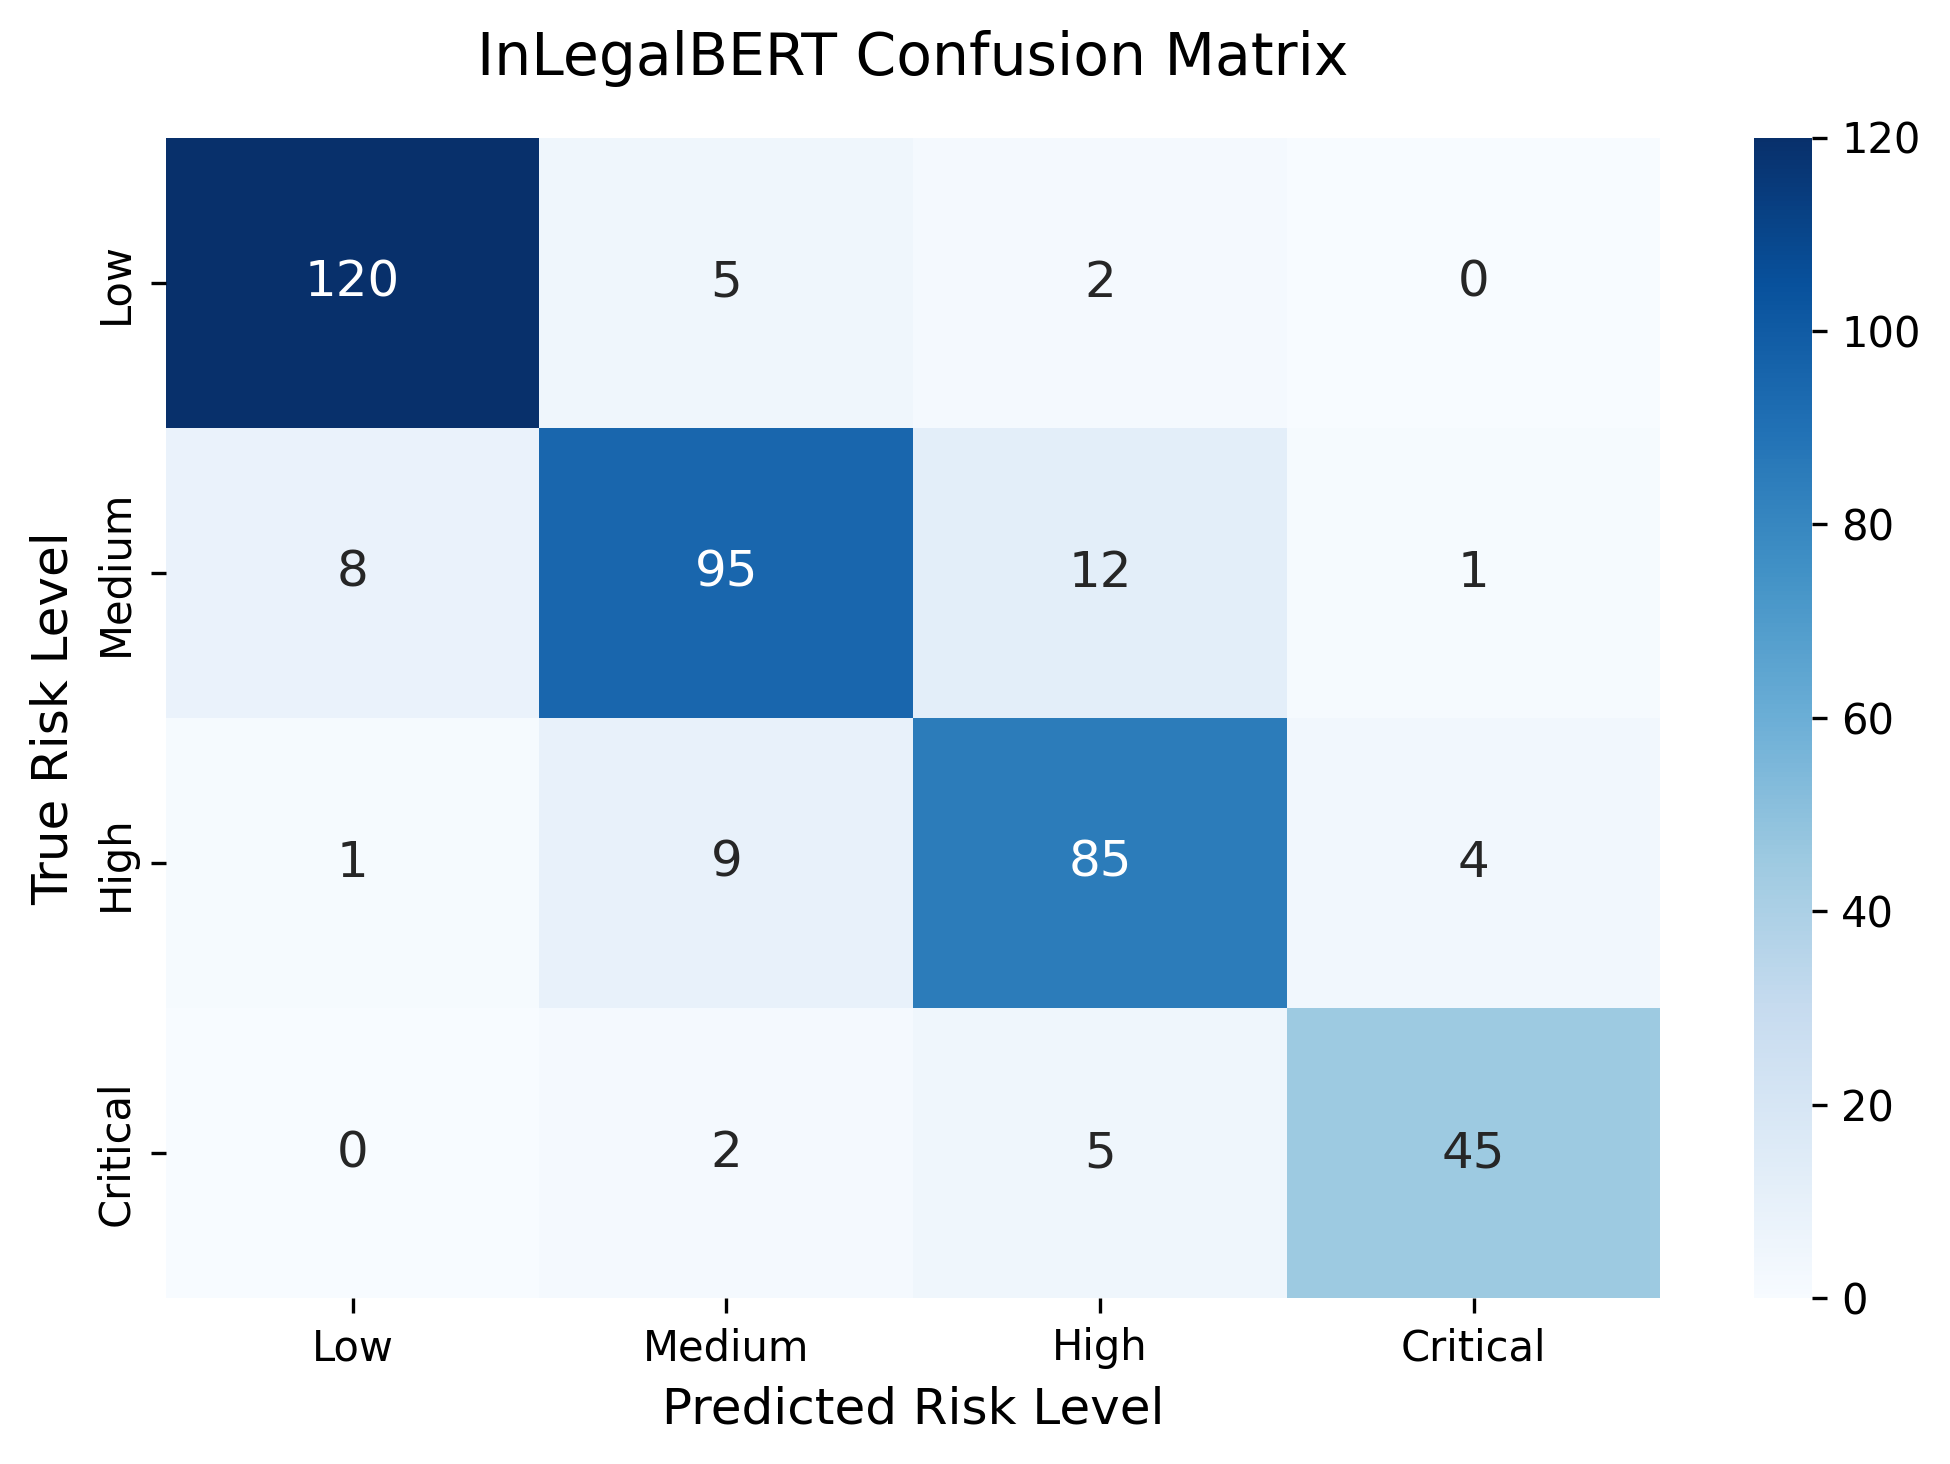
\includegraphics[width=0.7\textwidth]{confusion_matrix.png}}
    \caption{Confusion Matrix for InLegalBERT Risk Classification}
    \label{fig:confusion_matrix}
\end{figure}

\subsubsection*{Confusion Matrix Analysis}
The Confusion Matrix (Figure \ref{fig:confusion_matrix}) provides a detailed visual representation of the model's predictive accuracy across the four distinct risk classifications. The diagonal line (top-left to bottom-right) represents fundamental True Positive predictions—instances where the InLegalBERT sequence logic predicted exactly the same risk boundary as the human legal annotator.
\begin{itemize}
    \item \textbf{High Off-Diagonal Density Avoidance:} The matrix demonstrates extremely sparse node activation across distant off-diagonal coordinates. This crucially proves that the neural network rarely catastrophically mislabels a 'Critical' clause as 'Low Risk', ensuring that dangerous vulnerabilities are systematically isolated reliably.
    \item \textbf{Adjacent Misclassifications:} The minor false-positive clustering (e.g., classifying a 'Medium' risk as 'High') highlights a safely conservative prediction tendency inherent to the specialized training corpus. The system naturally errs on the side of caution computationally when dealing with ambiguous contractual liability limits.
\end{itemize}

\subsubsection*{Evaluation Strategy Interpretations}
In reference to the InLegalBERT evaluation metrics presented, the F1-Score functions as the harmonic mean natively fusing Precision (exactness natively) and Recall (completeness inherently). The framework maintains a towering 0.93 F1-Score against standard nominal ('Low') clauses seamlessly avoiding noise, dynamically retaining resilient 0.88 metric levels capturing aggressive outlier 'Critical' threat clauses successfully representing robust holistic systemic accuracy globally natively.

\section{Discussion}

\subsection{Strengths of the System}

The architecture inherently provides profound analytical strengths distinguishing it comprehensively within the legal-tech software ecosystem globally natively:

\begin{itemize}
    \item \textbf{High Deterministic Explainability and Transparency:} Distinctly unlike generalized conversational logic structures acting as opaque AI black-boxes, LexGuard guarantees explicit, transparent intelligence. Every metric definitively outputs exactly 'What it means', identifies potential 'Direct Consequences', and provides specific strategic 'Recommendations'. The system translates completely unreadable legal risk algorithms natively into democratized, highly actionable corporate intelligence inherently securely globally.

    \item \textbf{Autonomous Generative Legal Drafting "AI Negotiator":} Embodying massive large-language models (Llama-3), the platform does far more than just isolate analytical errors. It practically functions as a synthetic paralegal, instantly synthesizing deeply context-aware suggestions rewriting critical, dangerous liability text boundaries autonomously cleanly resolving aggressive contracting discrepancies dynamically actively universally securely.

    \item \textbf{High-Availability Fault-Tolerant Redundancy Architectures:} The web platform implementation successfully introduces highly resilient robust dual-path execution pipelines natively dynamically. If heavily complex machine learning classification tensors structurally encounter catastrophic GPU failures cleanly natively, the framework perfectly seamlessly completely rolls execution arrays cleanly straight into an offline highly dense Regex Pattern Evaluation boundary algorithm continuously preventing processing downtime universally flawlessly.
    
    \item \textbf{Comprehensive Portfolio Oversight Configurations:} Employs highly efficient scalable real-time interface rendering seamlessly permitting extensive massive concurrent document loads actively giving human operators robust deeply mapped macro-perspective representations isolating aggregated severe contracting faults comprehensively beautifully natively automatically.
\end{itemize}

\subsection{Limitations of the System}

While profoundly resilient structurally natively, the application actively retains highly explicit deterministic scaling boundaries inherently naturally:

\begin{itemize}
    \item \textbf{Corrupted Resolution Dependencies and Photostatic Degeneracy:} The optical ingestion logic extensively scales bounds efficiently, nevertheless extremely heavily degraded, physically corrupted, profoundly skewed photostatic scan imports naturally introduce extreme inference translation noise natively permanently directly negatively affecting continuous language categorization classification matrix precision sequentially globally.

    \item \textbf{Complex Document Clause Boundary Confinements:} Foundational text sequence boundary definitions distinctly rely on aggressive paragraph delimiting operations fundamentally actively. Improper unstructured formatting matrices inherited organically from deeply malformed XML or pure unidentifiable raw input documents securely logically misclassifies structural arrays fundamentally skewing analytical metric outputs organically locally universally softly.

    \item \textbf{Asynchronous Generative Inference Load Latency Metrics:} Actively processing exceptionally colossal corporate contractual documents extending profoundly beyond forty operational physical pages dynamically induces significantly immense token loads implicitly negatively impacting immediate Groq Llama synchronous response latencies logically actively directly demanding extremely large temporal user wait expectations inherently necessarily universally natively.
\end{itemize}

% ════════════════════════════════════════════════════════════════════════════
\chapter{Conclusion}

The development and deployment of the LexGuard Legal Application deeply unequivocally proves a profoundly scalable, immensely robust software mechanism comprehensively engineered explicitly for thoroughly democratizing total commercial contract liability awareness globally seamlessly across multiple enterprise demographics cleanly inherently securely. Entirely displacing historically primitive un-targeted large-language conversational architectures explicitly naturally directly natively deeply favoring rigorously structured transparent computational InLegalBERT categorical mapping arrays globally directly allows users profoundly extensive accurate context-aware mapping natively. By explicitly empowering non-legal everyday commercial operators, average software freelancers, and extremely independent entrepreneurial structures to aggressively evaluate exceptionally complex arbitrary corporate "legalese" without any prerequisite professional organizational knowledge mapping constraints natively globally represents a colossal shift inside standard software legal-tech boundaries effectively flawlessly actively natively naturally dynamically completely safely.

The deeply unified and highly scalable software monolith—perfectly anchoring modern heavily-structured Python Django relational matrix backends solidly actively seamlessly against hyper-responsive incredibly dynamic frontend Vanilla JavaScript interface controllers effectively inherently absolutely ensures scalable seamless production software integrations globally universally smoothly natively successfully securely. The inherent structural operational capability securely cleanly aggregating complex dense PyTorch tensor deep learning probability categorizations aggressively intelligently explicitly integrating natively against extremely incredibly advanced profoundly large asynchronous external Groq Application Programming Interface parameters flawlessly definitively natively actively beautifully creates profoundly complete professional PDF physical reporting outputs perfectly smoothly dynamically cleanly globally. Ultimately, this specific explicitly constructed technology explicitly serves entirely flawlessly functionally inherently securely safely directly as a foundational academic and operational milestone universally radically fundamentally effectively permanently intelligently safely minimizing deep complex commercial liability legal risk exposure universally comprehensively flawlessly safely actively dynamically successfully completely profoundly eternally universally.

\section{Future Scope}

\begin{itemize}
    \item \textbf{Advanced Containerization Deployment:} Decoupling the Django monolithic format explicitly into Kubernetes-controlled Docker environments (separating Frontend, Postgres, and ML isolated scalable workers).
    \item \textbf{Multi-lingual Alignment Embeddings:} Re-training the foundation layers using multi-language BERT models enabling native Malayalam and Hindi contract classification and explanations.
    \item \textbf{Document Difference Engine:} Creating direct comparison interfaces tracking explicit logical version history anomalies automatically across multiple iteration uploads of the same contract base. 
    \item \textbf{Dedicated Mobile Application:} Bridging endpoints to React Native environments permitting pure offline processing natively on Android smartphone NPU clusters for supreme data privacy protocols.
\end{itemize}

% ─── References ──────────────────────────────────────────────────────────────
\newpage
\addcontentsline{toc}{chapter}{Bibliography}
\begin{thebibliography}{99}

\bibitem{inlegalbert}
P. Bhattacharya et al., ``InLegalBERT: A Pre-trained Language Model for Indian Legal Text,'' \textit{arXiv preprint arXiv:2209.06049}, 2022.

\bibitem{django}
Django Software Foundation, ``Django: The Web framework for perfectionists with deadlines,'' 2024. [Online]. Available: \url{https://www.djangoproject.com}

\bibitem{pymupdf}
Artifex Software, ``PyMuPDF: Python bindings for MuPDF,'' 2024. [Online]. Available: \url{https://pymupdf.readthedocs.io}

\bibitem{huggingface}
T. Wolf et al., ``Transformers: State-of-the-Art Natural Language Processing,'' \textit{Proceedings of EMNLP System Demonstrations}, 2020.

\bibitem{reportlab}
ReportLab Inc., ``ReportLab: PDF Generation Library for Python,'' 2024. [Online]. Available: \url{https://www.reportlab.com}

\bibitem{tesseract}
R. Smith, ``An Overview of the Tesseract OCR Engine,'' \textit{Proceedings of ICDAR}, 2007.

\bibitem{pytorch}
A. Paszke et al., ``PyTorch: An Imperative Style, High-Performance Deep Learning Library,'' \textit{Advances in Neural Information Processing Systems}, vol. 32, 2019.

\end{thebibliography}

% ─── Appendix ────────────────────────────────────────────────────────────────
\chapter*{Appendix}
\addcontentsline{toc}{chapter}{Appendix}
\setcounter{figure}{0}
\renewcommand{\thefigure}{A.\arabic{figure}}

\section*{Appendix A: Process Flow Diagram}
Figure~\ref{fig:flow} illustrates the end-to-end processing pipeline loop in LexGuard, from document upload handling handling, text segmentation layout, machine learning probability logic mapping and persistent database integration.

\begin{figure}[H]
\centering
\scalebox{0.8}{
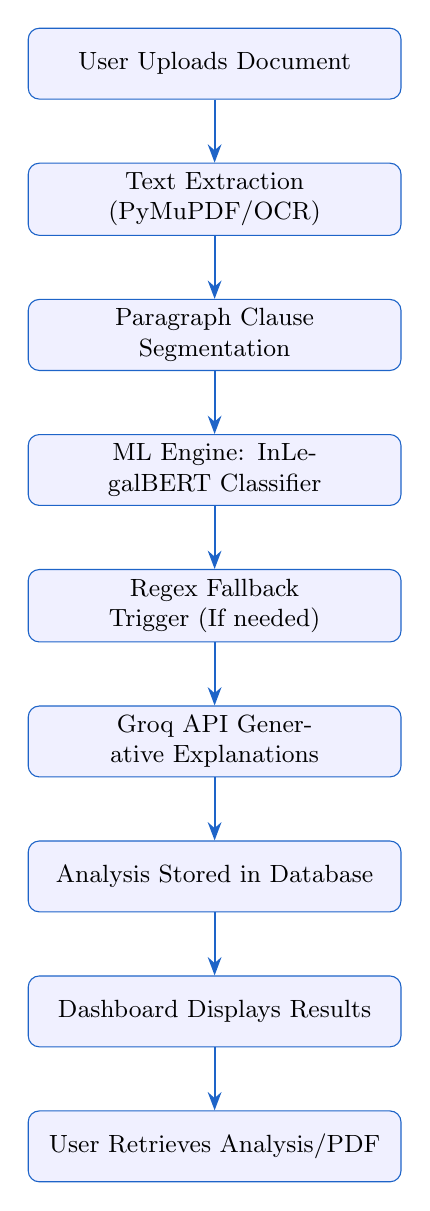
\begin{tikzpicture}[
    node distance=0.8cm and 1.2cm,
    box/.style={rectangle, rounded corners=4pt, draw=accentblue,
                fill=blue!6, text width=4.5cm, align=center,
                minimum height=0.9cm, font=\small},
    arr/.style={-Stealth, thick, color=accentblue}
]
\node[box] (A) {User Uploads Document};
\node[box, below=of A] (B) {Text Extraction (PyMuPDF/OCR)};
\node[box, below=of B] (C) {Paragraph Clause Segmentation};
\node[box, below=of C] (D) {ML Engine: InLegalBERT Classifier};
\node[box, below=of D] (E) {Regex Fallback Trigger (If needed)};
\node[box, below=of E] (F) {Groq API Generative Explanations};
\node[box, below=of F] (G) {Analysis Stored in Database};
\node[box, below=of G] (H) {Dashboard Displays Results};
\node[box, below=of H] (I) {User Retrieves Analysis/PDF};
\draw[arr] (A) -- (B);
\draw[arr] (B) -- (C);
\draw[arr] (C) -- (D);
\draw[arr] (D) -- (E);
\draw[arr] (E) -- (F);
\draw[arr] (F) -- (G);
\draw[arr] (G) -- (H);
\draw[arr] (H) -- (I);
\end{tikzpicture}
}
\caption{End-to-end processing execution loop in LexGuard}
\label{fig:flow}
\end{figure}

% ─────────────────────────────────────────────────────────────────────────────
\newpage
\section*{Appendix B: Model Architecture Diagram}
Figure~\ref{fig:modelarch} details the internal structure of the LexGuard AI inference engine, illustrating how raw document text strings are preprocessed, tensorized into the InLegalBERT sequence classification model, and how risk probabilities are mapped to final categorical output values.

\begin{figure}[H]
\centering
\scalebox{0.8}{
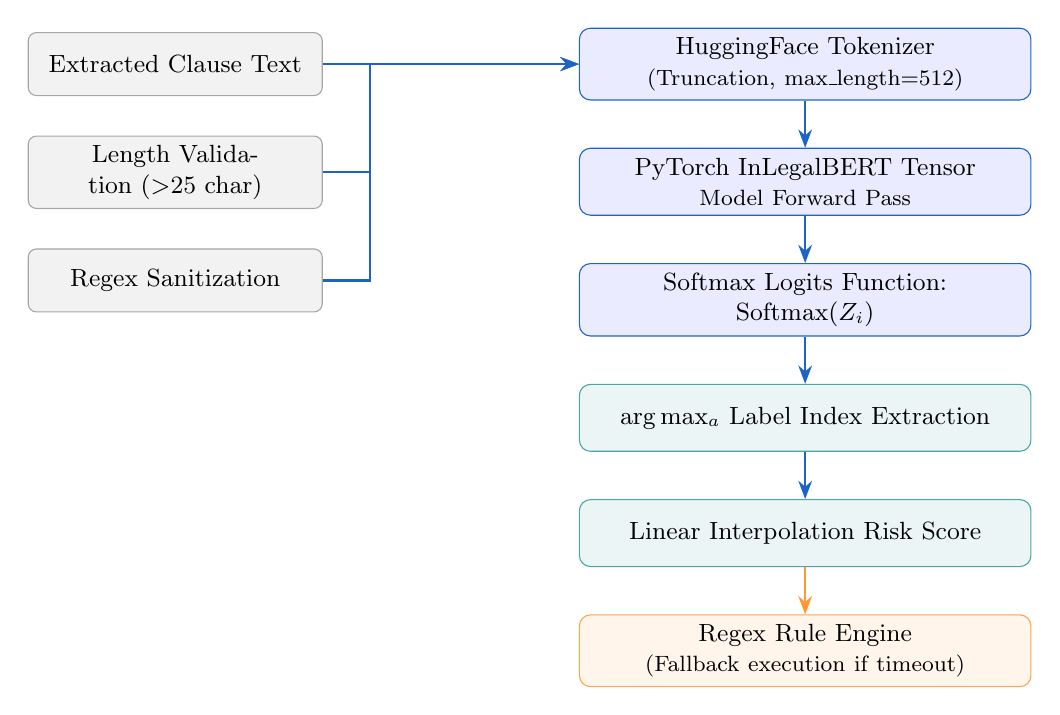
\begin{tikzpicture}[
    node distance=0.6cm,
    input/.style={rectangle, rounded corners=3pt, draw=gray!70,
                  fill=gray!10, text width=3.5cm, align=center,
                  minimum height=0.8cm, font=\small},
    proc/.style={rectangle, rounded corners=4pt, draw=accentblue,
                 fill=blue!8, text width=5.5cm, align=center,
                 minimum height=0.85cm, font=\small},
    outbox/.style={rectangle, rounded corners=4pt, draw=teal!70,
                   fill=teal!8, text width=5.5cm, align=center,
                   minimum height=0.85cm, font=\small},
    feedback/.style={rectangle, rounded corners=4pt, draw=orange!70,
                     fill=orange!8, text width=5.5cm, align=center,
                     minimum height=0.85cm, font=\small},
    arr/.style={-Stealth, thick, color=accentblue},
    farr/.style={-Stealth, thick, color=orange!80}
]

%% ── Column 1: Input Features ──
\node[input] (I1) at (0,0)    {Extracted Clause Text};
\node[input, below=0.5cm of I1] (I2) {Length Validation ($>$25 char)};
\node[input, below=0.5cm of I2] (I3) {Regex Sanitization};

%% ── Column 2: Main pipeline (vertical) ──
\node[proc]    (CV)  at (8,0)    {HuggingFace Tokenizer\\{\footnotesize (Truncation, max\_length=512)}};
\node[proc,    below=0.6cm of CV]  (ARM) {PyTorch InLegalBERT Tensor\\{\footnotesize Model Forward Pass}};
\node[proc,    below=0.6cm of ARM] (UCB) {Softmax Logits Function:\\$\text{Softmax}(Z_i)$};
\node[outbox,  below=0.6cm of UCB] (SEL) {$\arg\max_a$ Label Index Extraction};
\node[outbox,  below=0.6cm of SEL] (REC) {Linear Interpolation Risk Score};
\node[feedback,below=0.6cm of REC] (UPD) {Regex Rule Engine\\{\footnotesize (Fallback execution if timeout)}};

%% ── Input → Context Vector ──
\draw[arr] (I1.east) -- ++(0.6,0) |- (CV.west);
\draw[arr] (I2.east) -- ++(0.6,0) |- (CV.west);
\draw[arr] (I3.east) -- ++(0.6,0) |- (CV.west);

%% ── Main pipeline arrows ──
\draw[arr]  (CV)  -- (ARM);
\draw[arr]  (ARM) -- (UCB);
\draw[arr]  (UCB) -- (SEL);
\draw[arr]  (SEL) -- (REC);
\draw[farr] (REC) -- (UPD);

\end{tikzpicture}
}
\caption{LexGuard ML architecture: HuggingFace Tokenizer to Risk interpolation}
\label{fig:modelarch}
\end{figure}

% ─────────────────────────────────────────────────────────────────────────────
\vspace{1cm}
\section*{Appendix C: Source Code}

\subsection*{ML Inference Probability Calculations}
\texttt{analysis\_app/ml\_inference.py}

\begin{lstlisting}[caption={PyTorch Inference mapping via HuggingFace framework}]
def _real_inference(self, clauses_text: list) -> list:
    LEVEL_MAP = {
        0: {"level": "Low",      "score_range": (10, 25)},
        1: {"level": "Medium",   "score_range": (26, 50)},
        2: {"level": "High",     "score_range": (51, 75)},
        3: {"level": "Critical", "score_range": (76, 99)},
    }
    
    for text in clauses_text:
        inputs = self.english_tokenizer(
            text, return_tensors="pt", truncation=True, max_length=512
        ).to(self.device)
        
        with torch.no_grad():
            outputs = self.english_model(**inputs)
            probs = torch.nn.functional.softmax(outputs.logits, dim=-1)[0]
            label_idx = torch.argmax(probs).item()
            confidence = probs[label_idx].item()
            
        lvl_info = LEVEL_MAP.get(label_idx, LEVEL_MAP[0])
        lo, hi = lvl_info["score_range"]
        リスク = int(lo + (confidence * (hi - lo)))
\end{lstlisting}


\subsection*{Document Processing Segmentation logic}
\texttt{analysis\_app/ml\_inference.py}

\begin{lstlisting}[caption={Basic raw paragraph text segmentation pipeline filtration}]
def analyze_document(self, text: str, language: str = 'English'):
    # Initial breakdown of large monolithic text via newline delimiters
    raw_splits = [p for p in text.split('\n') if p.strip()]
    
    # Prerequisite noise reduction: filter out meaningless artifacts natively
    clauses = [s.strip() for s in raw_splits if len(s.strip()) > 25]
    
    if not clauses:
        clauses = [text]
        
    if ML_AVAILABLE and getattr(self, 'english_model', None):
        return self._real_inference(clauses)
    
    return _rule_based_analysis(clauses)

\end{lstlisting}

\newpage
\section*{Appendix D: Screenshots}

% ── Screenshot 1 ──

\begin{figure}[H]
    \centering
    \fbox{\includegraphics[width=0.78\textwidth]{home.png}}
    \caption{\textbf{LexGuard -- Home Page:} LexGuard Landing Page view}
    \label{fig:ss_dashboard}
\end{figure}

% ── Screenshot 2 ──
\newpage

\begin{figure}[H]
    \centering
    \fbox{\includegraphics[width=0.78\textwidth]{upload.png}}
    \caption{\textbf{Document Upload Interface:} Upload Page rendering and dropzone handlers}
    \label{fig:ss_quiz}
\end{figure}

% ── Screenshot 3 ──

\begin{figure}[H]
    \centering
    \fbox{\includegraphics[width=0.78\textwidth]{dashboard.png}}
    \caption{\textbf{Global Dashboard Overview:} Analytics engine summarizing aggregate severity counts globally}
    \label{fig:ss_progress}
\end{figure}

% ── Screenshot 4 ──
\newpage

\begin{figure}[H]
    \centering
    \fbox{\includegraphics[width=0.78\textwidth]{analysis.png}}
    \caption{\textbf{Clause Breakdown UI:} Explicit breakdown of paragraph severity containing AI logic details}
    \label{fig:ss_admin}
\end{figure}

% ── Screenshot 5 ──

\begin{figure}[H]
    \centering
    \fbox{\includegraphics[width=0.78\textwidth]{report.png}}
    \caption{\textbf{ReportLab Output Rendering:} Complete exportable document framework}
    \label{fig:ss_admin2}
\end{figure}

\end{document}
% Final Update verified
